\begin{figure}[htbp]
  \begin{tabular}{ccc}
    \begin{minipage}{0.33\hsize}
      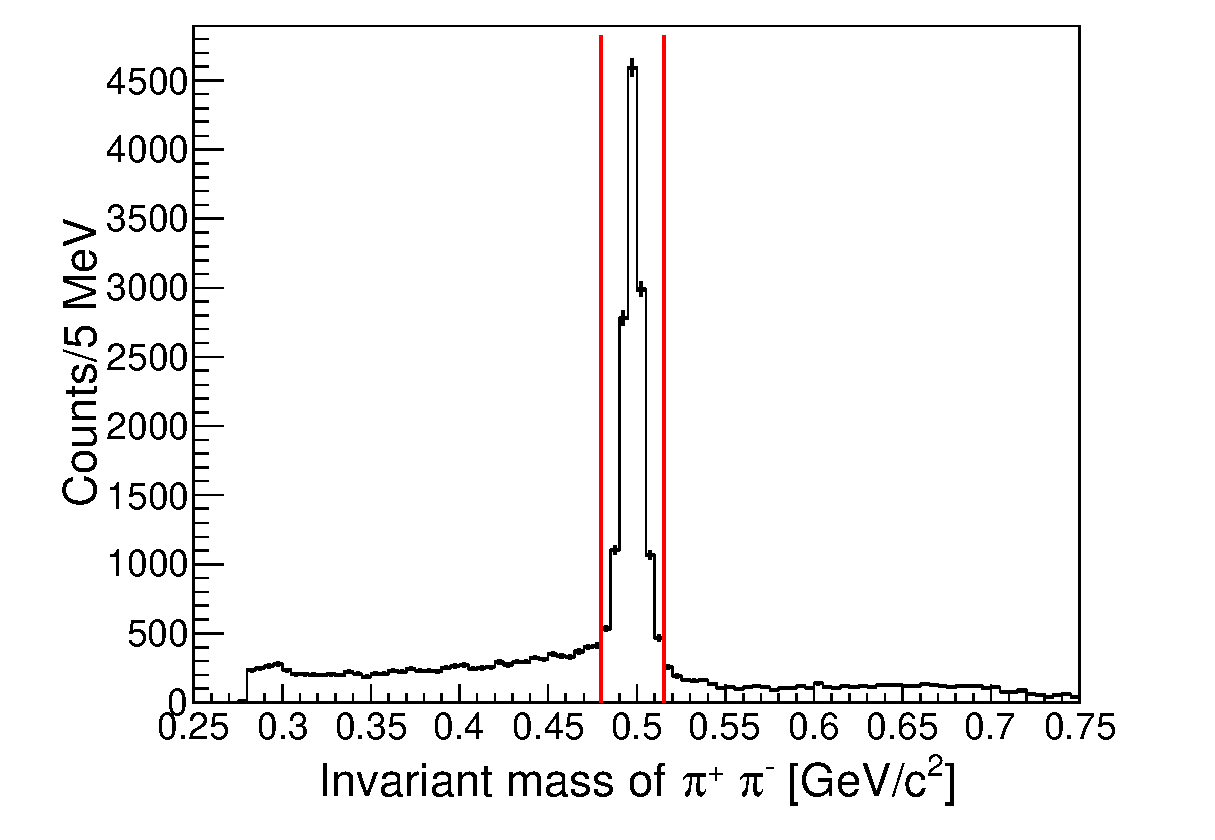
\includegraphics[width=4cm]{../pic/Run78/KN_ana_NC170_2sigma/IM_pipi_woFit.eps}
    \end{minipage}
    \begin{minipage}{0.33\hsize}
      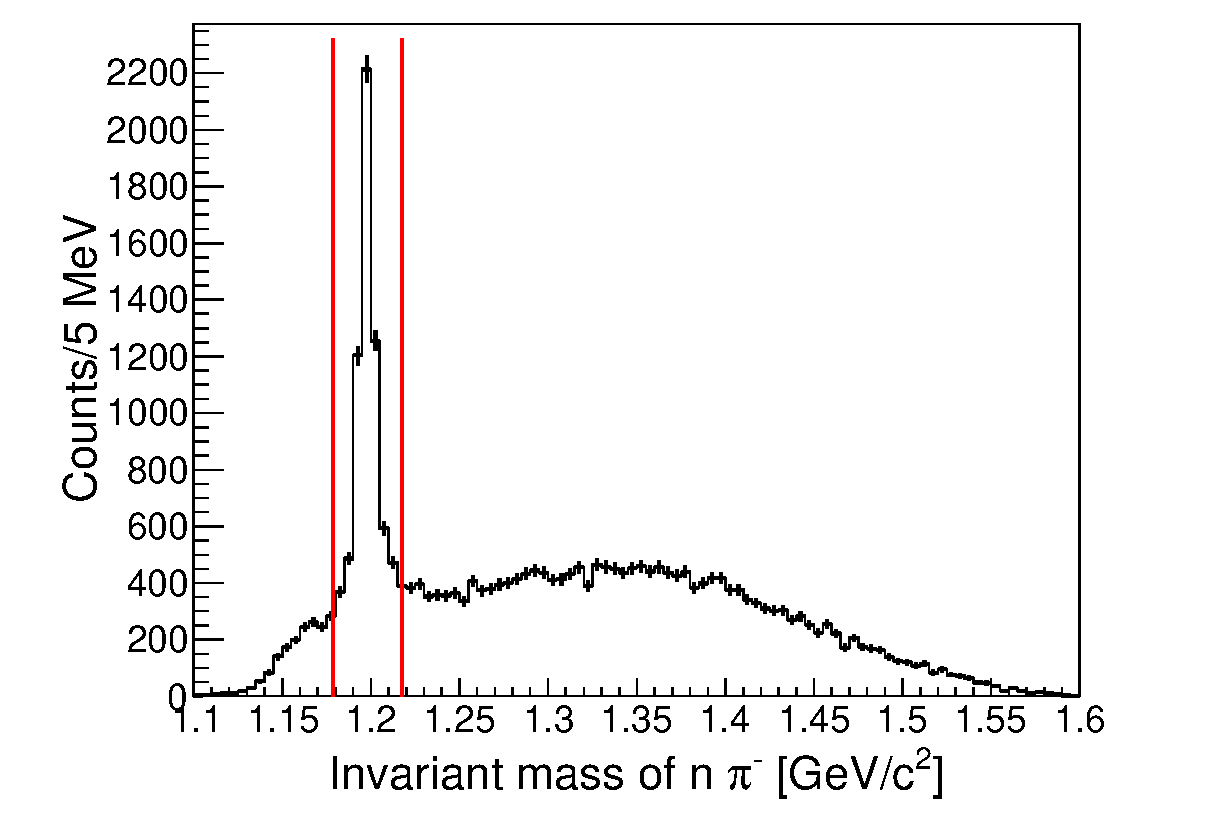
\includegraphics[width=4cm]{../pic/Run78/KN_ana_NC170_2sigma/IM_npim_woFit.eps}
    \end{minipage}
    \begin{minipage}{0.33\hsize}
      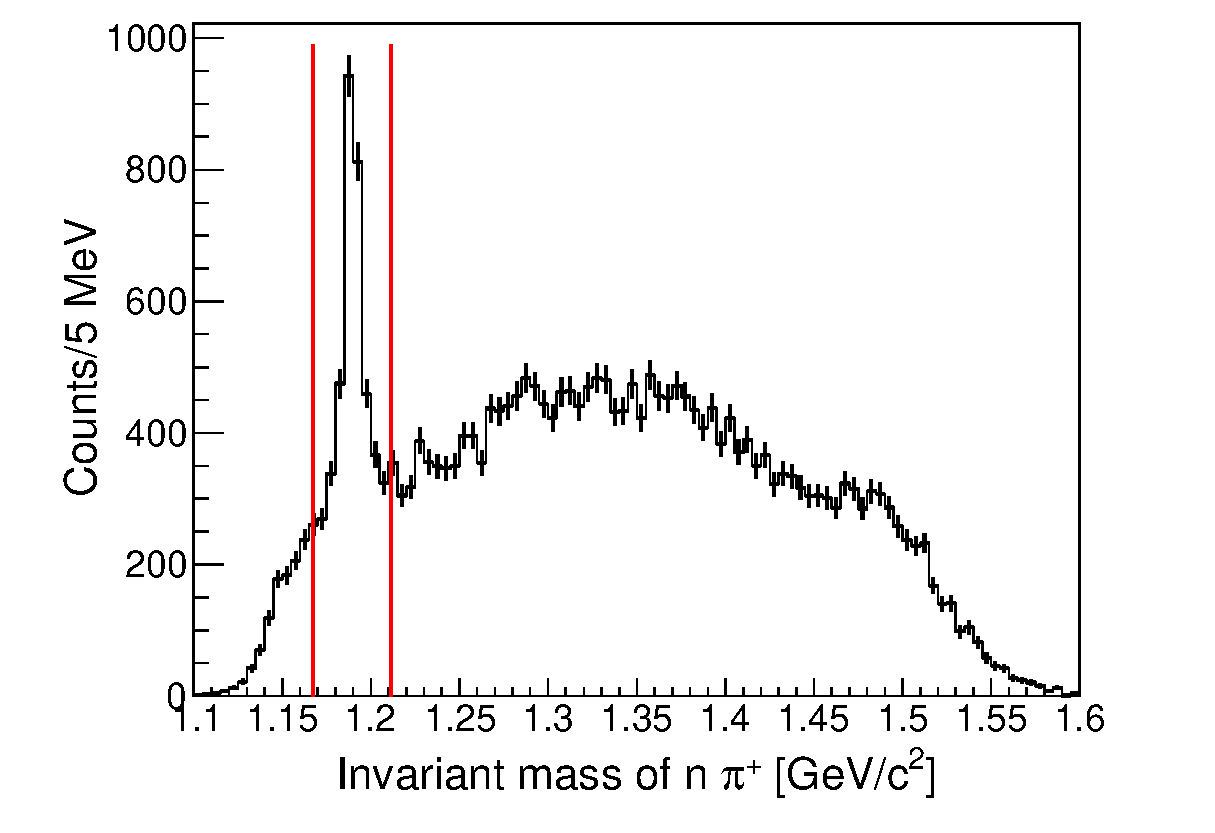
\includegraphics[width=4cm]{../pic/Run78/KN_ana_NC170_2sigma/IM_npip_woFit.eps}
    \end{minipage}
  \end{tabular}

  \caption{
    These figures show invariant masses of $\pi^+ \pi^-$, $n \pi^-$ and $n \pi^+$ in $K^- d \rightarrow n \pi^+ \pi^- n$ final state identified events, respectively.
    Red lines indicate select region for $K^0$, $\Sigma^-_{forward}$ and $\Sigma^+_{backward}$, respectively.
  }
  \label{fig:KNpipi_IM}
\end{figure}
